\documentclass[10pt]{article}
\usepackage[margin=0.7in]{geometry}
\usepackage{booktabs,graphicx,hyperref}
\title{Fixed-offset Kummer sidecar orbit bounds}
\author{Study KUMMER-FIXED-OFFSET-ORBIT-20261024}
\date{24 October 2026}
\begin{document}
\maketitle
\noindent This proof-and-derivation run uses 21 frozen prime-order groups and
16 canonical nonzero jumps per group. It executes no target and performs no
scalar recovery.

\begin{center}
\begin{tabular}{lr}
\toprule
Recorded quantity & Result\\
\midrule
Models / jumps / bound rows & 21 / 16 / 336\\
Standard price rows & 12,096\\
Exact full-order orbit rows & 336 / 336\\
Minimum logical offsets & 34,147--552,130,504,327\\
Current explicit state (bytes) & 1,092,704--17,668,176,138,464\\
Regular cached-xADD bound (M-equivalent) & 819,528--13,251,132,103,848\\
Native validator failures & 0\\
\bottomrule
\end{tabular}
\end{center}

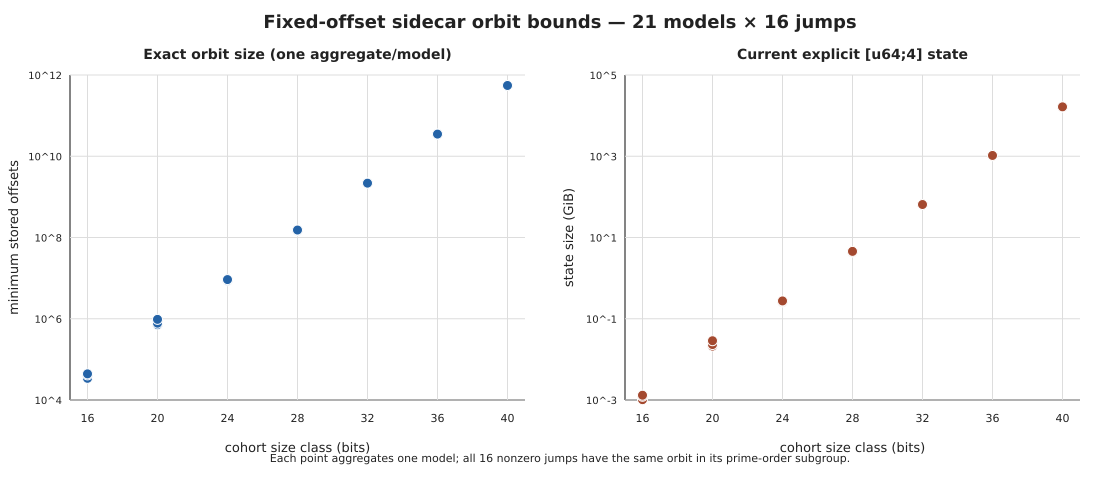
\includegraphics[width=0.97\textwidth]{orbit-bounds.png}

\paragraph{Statement and scope.}
If a nonempty state explicitly stores $K(T+s)$ and a direct one-xADD update
after fixed jump $J$ requires the predecessor offset, closure under $s\mapsto
s-J$ contains the whole translation orbit. Lean proves this conditional
closure theorem. The native validator checks that every frozen subgroup order
is prime and every jump scalar is nonzero and coprime to it, so all 336 orbit
sizes equal $r$.

  Storage uses the current Rust \texttt{[u64;4]} representation. Update cost
  uses 24 field multiplications and 36 field additions for one regular cached
xADD per entry. These are representation- and recurrence-specific bounds, not
a full collector price or a rho comparison. Compressed states,
project-pseudomultiply-recover chains, label-free recurrences, variable-offset
sidecars, and different walks remain outside the theorem.

\paragraph{Artifacts.}
The packet contains the frozen JSON input, 336-row bounds, 12,096-row price
grid, independent validation receipt, graph, theorem source, proof-gate log,
manifest, and SHA-256 list. The manifest pins the complete input digest.
\end{document}
